\chapter{Analysis }
It is hypothesized that the size of a Bombus Terrestris has an impact on its behavior (cite Emily et al). In particular, it is likely that this difference in behavior translates to a difference in the shape of the eyes of Bombus Terrestris. We investigate this hypothesis as a means of showcasing the use of persistent homology in the wild in order to see whether the topological summaries given by persistent homology support this hypothesis.
\subsection{Data}
The data consists of binary 3D volumes of the corneas acquired by microCT scans of different species. The main focus of the analysis will be Bombus Terrestris, but in total there are 20 samples consisting of ? different species. We use the additional samples to act as a control upon our topological findings. See figure ? for a full breakdown of the samples.
\subsection{Methodology}
Since our samples consist of binary 3D volumes they can be considered as cubes in a 3-dimensional grid, where a value of $1$ indicates the presence of a cube and a value of $0$ indicates the absence of one. We can exploit this inherent structure in the data and instead of considering simplicial complexes as described in Section ? we can instead impose the structure of a \textit{cubical complex} on the data samples. The benefits are computational.

\subsubsection{Cubical complexes}
Describe cubical complexes. Describe how they work. Describe how nothing changes other than the complex construction: from there on the results and definitions regarding persistent homology are the same.

Lore
Lore
Lorem ipsum.

We also need to impose a metric structure on the space given by each sample. If we only consider the binary situation then threshold in which persistent homology examines the sample will just lead to all cubes appearing at a threshold of $1$. Instead, we consider the Euclidean Distance Transform (EDT).

\begin{definition}
  The Euclidean Distance Transform is a function from $Z \times Z \to \mathbb{R} \times \mathbb{R}$ in the following way: Give each n-dimensional cube a value depending on how far away it is from the background (where values are 0).
\end{definition}

2-dimensional example here.

In order for not all topological features to appear at the same time we slightly perturb each value with some random uniform noise. In Figure ? we see what the sample ??? looks like at different thresholds.

Our filtration then, as the threshold increases, will describe the structure starting at the densest parts of the cornea and expanding until the entire cornea is considered. The resulting barcode then describes to us the local geometries and the innermost levels of the cornea as well as the global topology when the entire cornea is considered. Our reason for doing this is because the cornea considered as a whole has a trivial topology: it has no holes and consists of a single connected component. But this allows us to look at it at different scales.

The resulting topological summaries we find are barcodes. While these are in themselves interesting, in order to answer whether the size of a Bombus Terrestris has an impact on the topology of its cornea we compare the samples in a distance matrix where the metric is the 1-Wasserstein distance. We choose the Wasserstein distance because it is sensitive to small changes in the persistence diagrams whereas the bottleneck distance only considers the largest differences.

We then analyze this distance matrics using standard tools for data analysis. We are interested in two things:
\begin{enumerate}
  \item is there a correlation between the size of the bumblebees and their persistent homology?
  \item is persistent homology able to identify subgroups of bumblebees, and if so is it related to their size?
\end{enumerate}
Answering these questions will allow us to evaluate whether persistent homology provides information which relates to the hypothesis. In order to check the correlation we additionally compute the distance matrix between the samples' ITW (whatever this abbreviated, the size between wings in insect morphology) and use the Mantel test to see the correlation between the wasserstein distance matrix (describe mantel test). In order to identify groupings in the samples we use hierarchical clustering (describe this as well).
\subsection{Results}
\begin{figure}[ht]
  \centering
  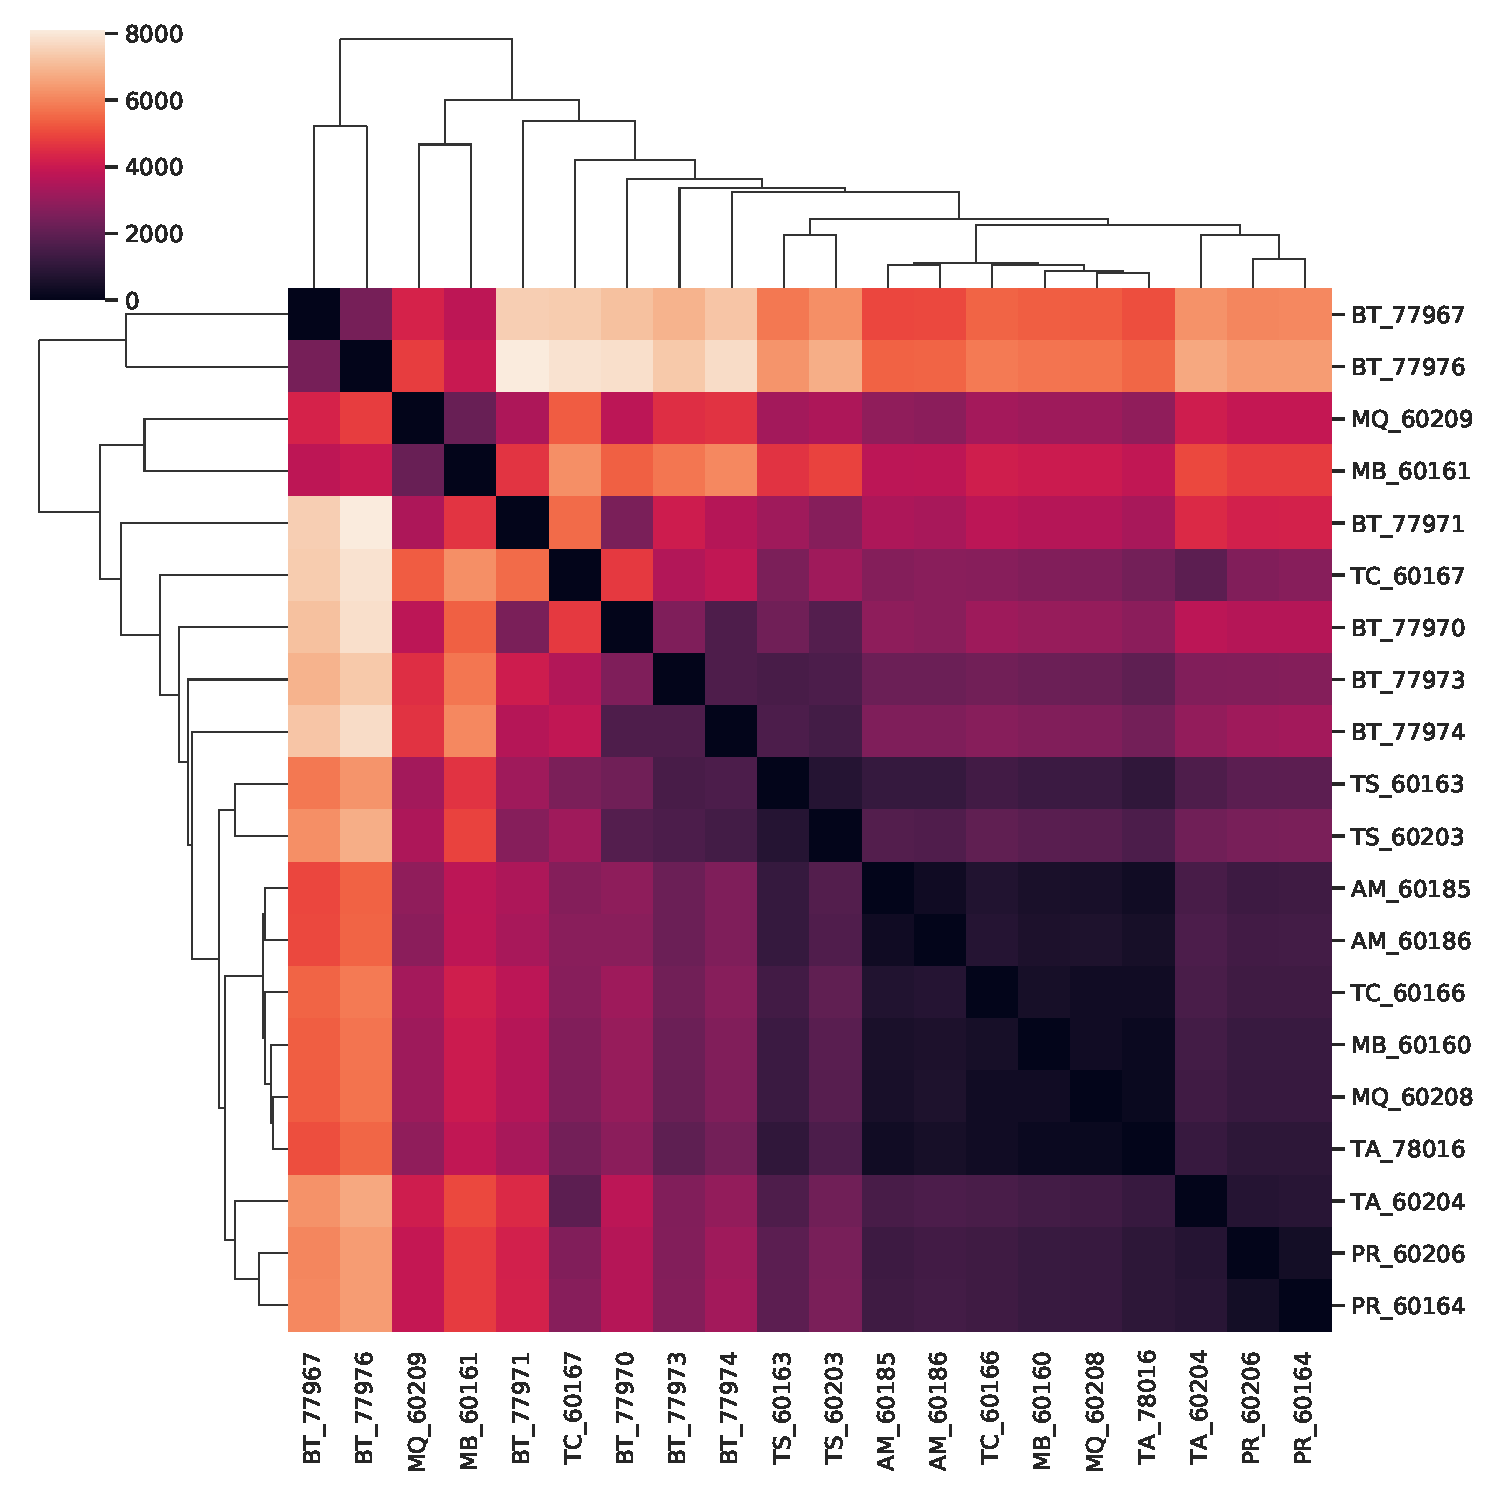
\includegraphics[scale=0.35]{clusters/wasserstein_h1_full.pdf}
  \caption{\label{fig:label} }
\end{figure}



\begin{figure}[ht]
  \centering
  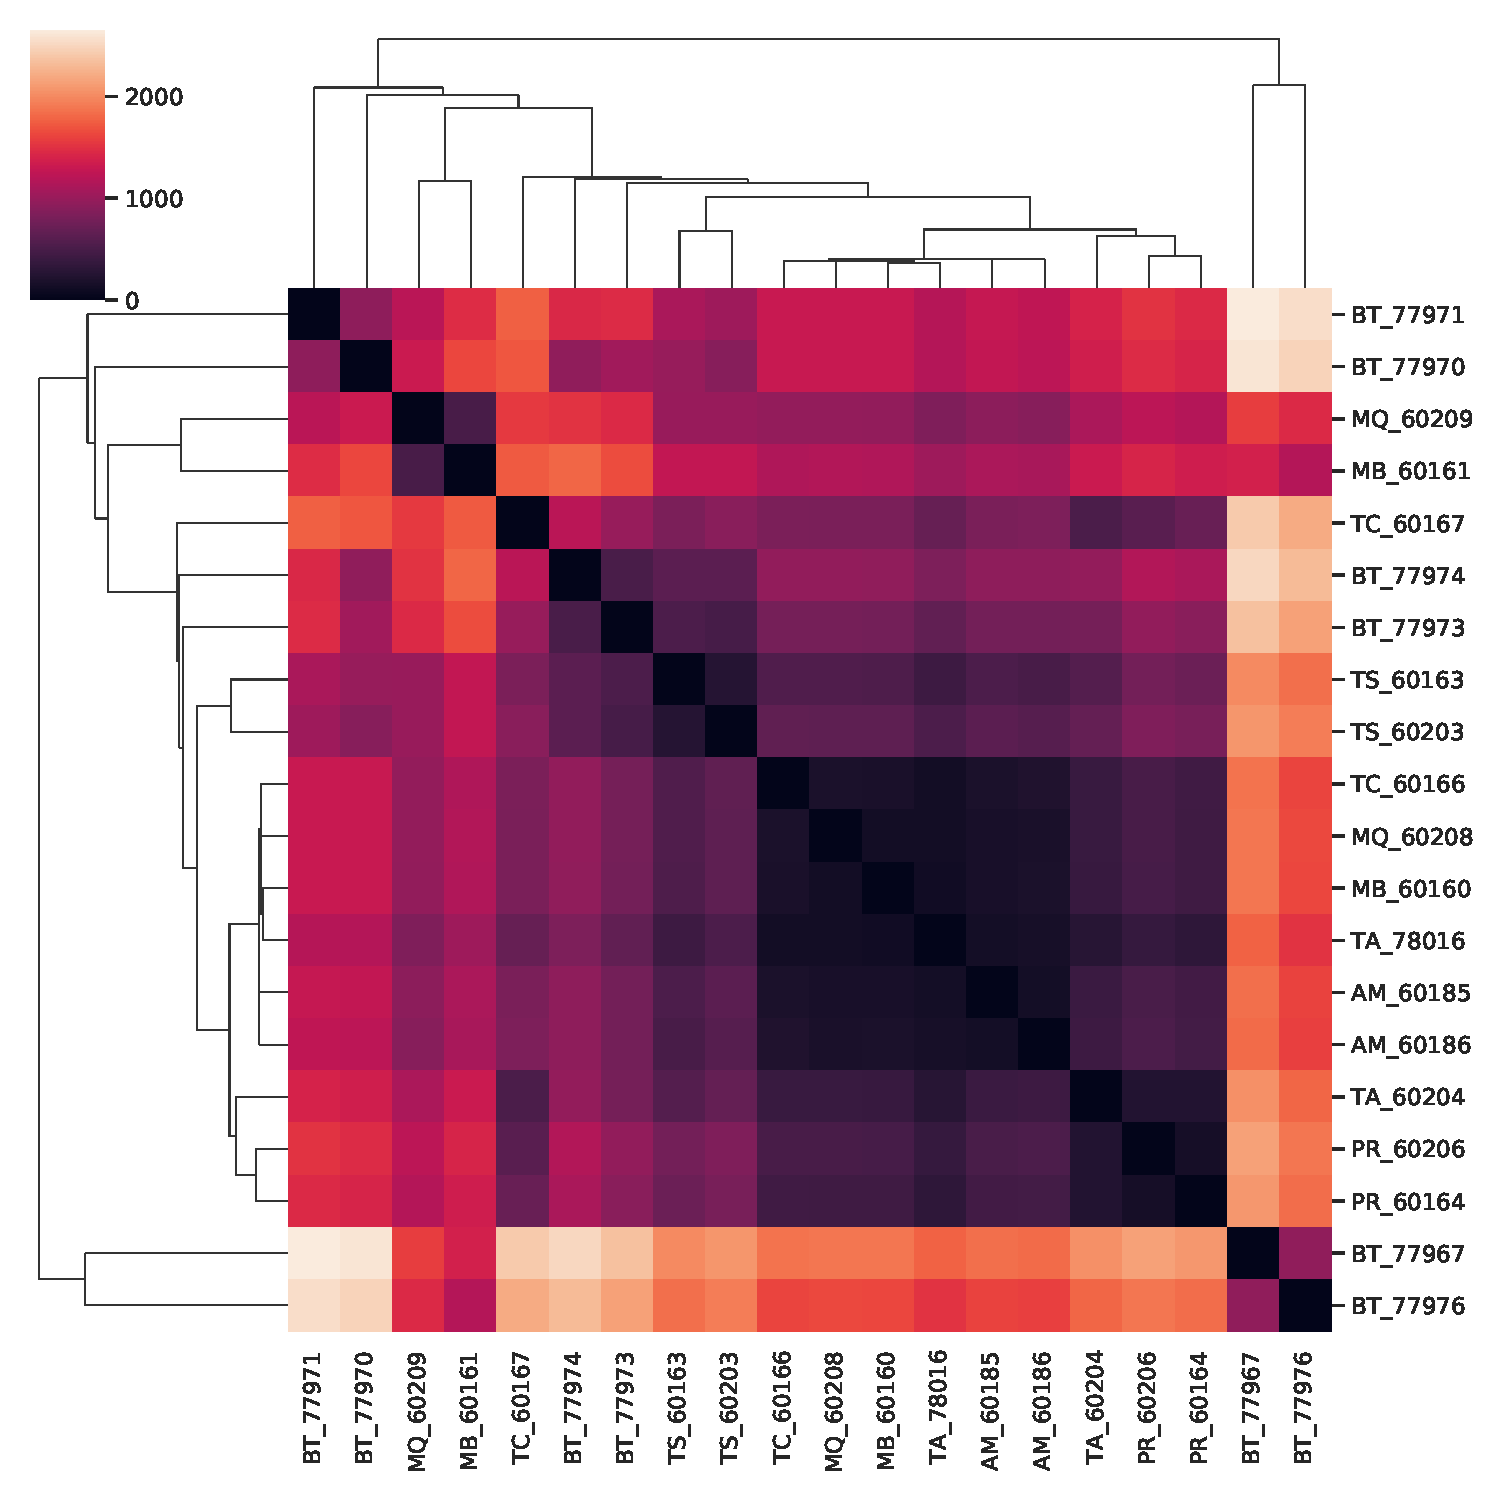
\includegraphics[scale=0.35]{clusters/wasserstein_h2_full.pdf}
  \caption{\label{fig:label} }
\end{figure}

\begin{figure}[ht]
  \centering
  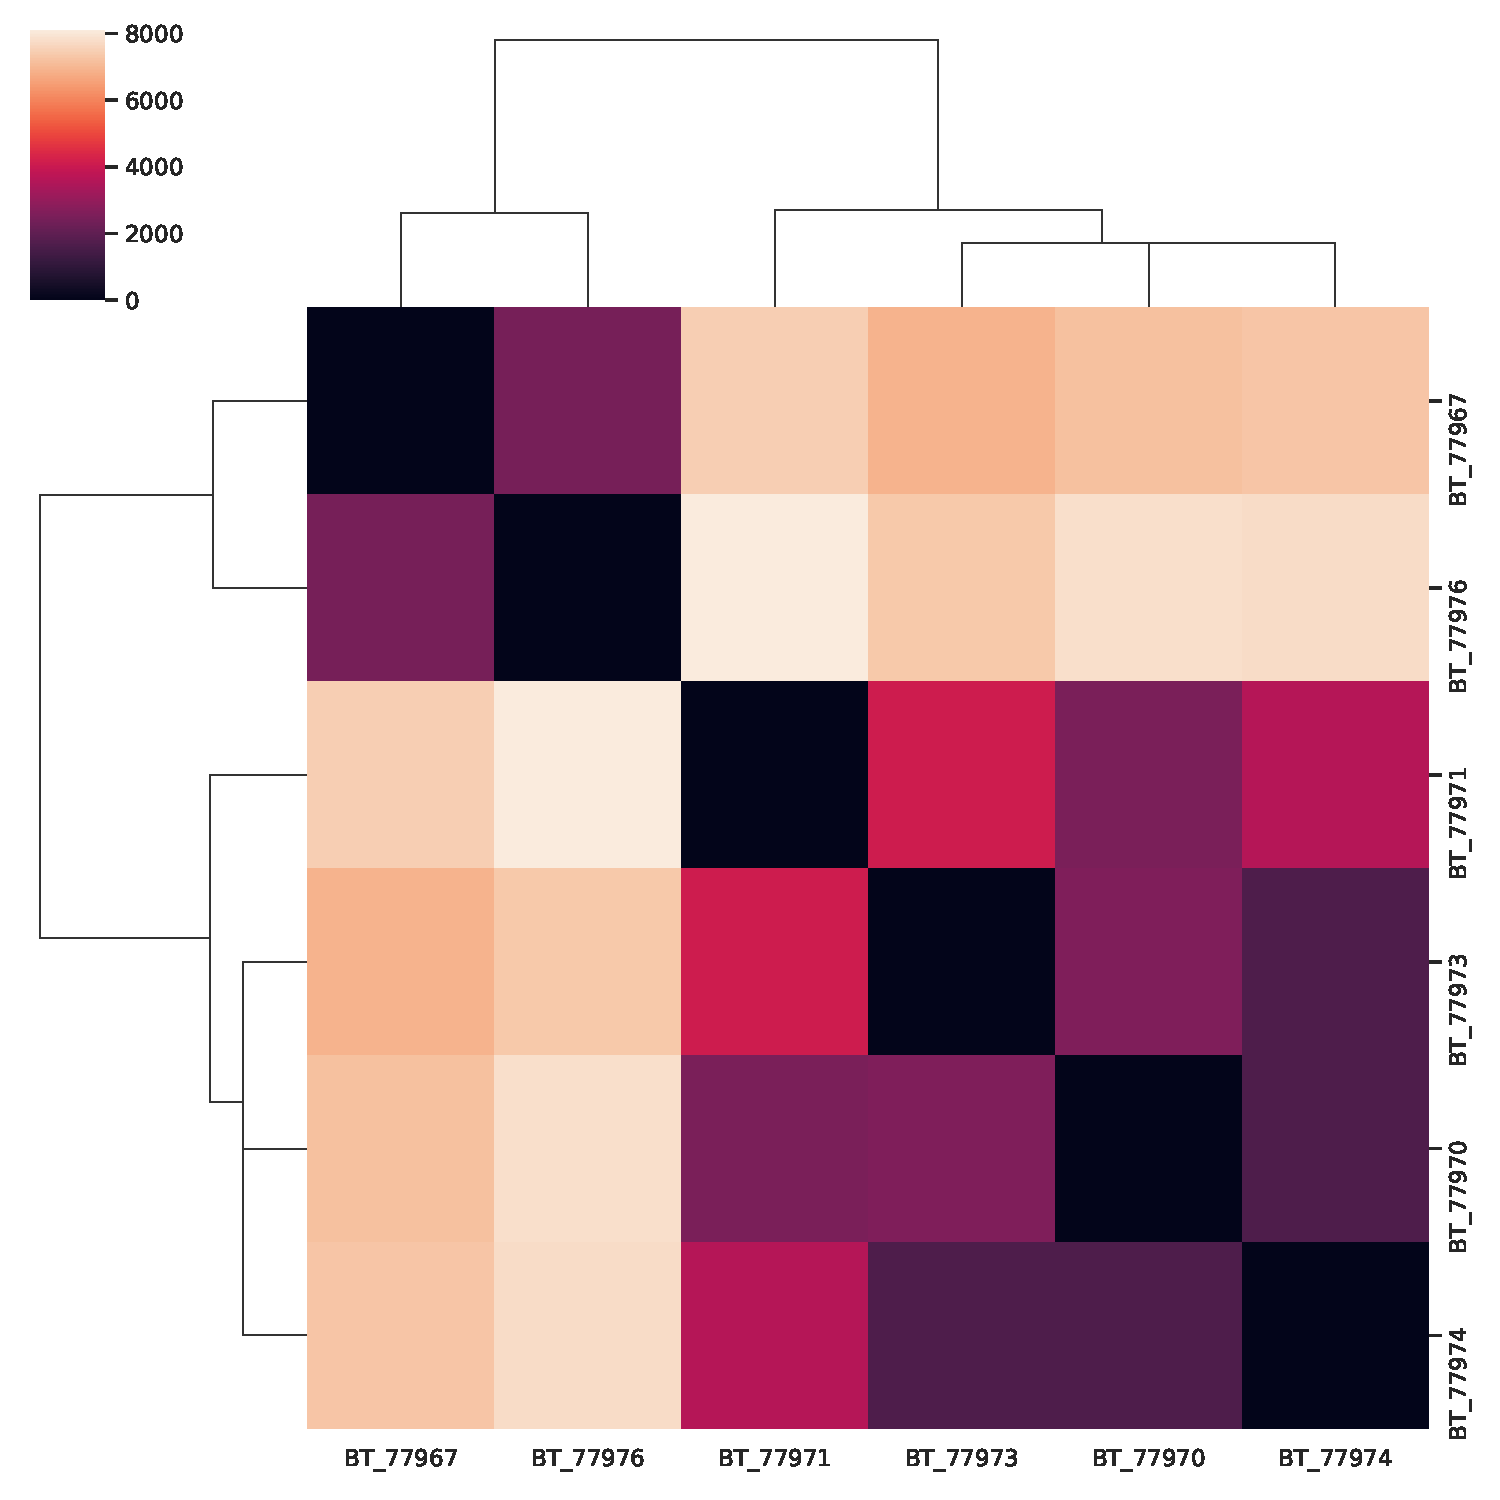
\includegraphics[scale=0.35]{clusters/wasserstein_h1_bt.pdf}
  \caption{\label{fig:label} }
\end{figure}

\begin{figure}[ht]
  \centering
  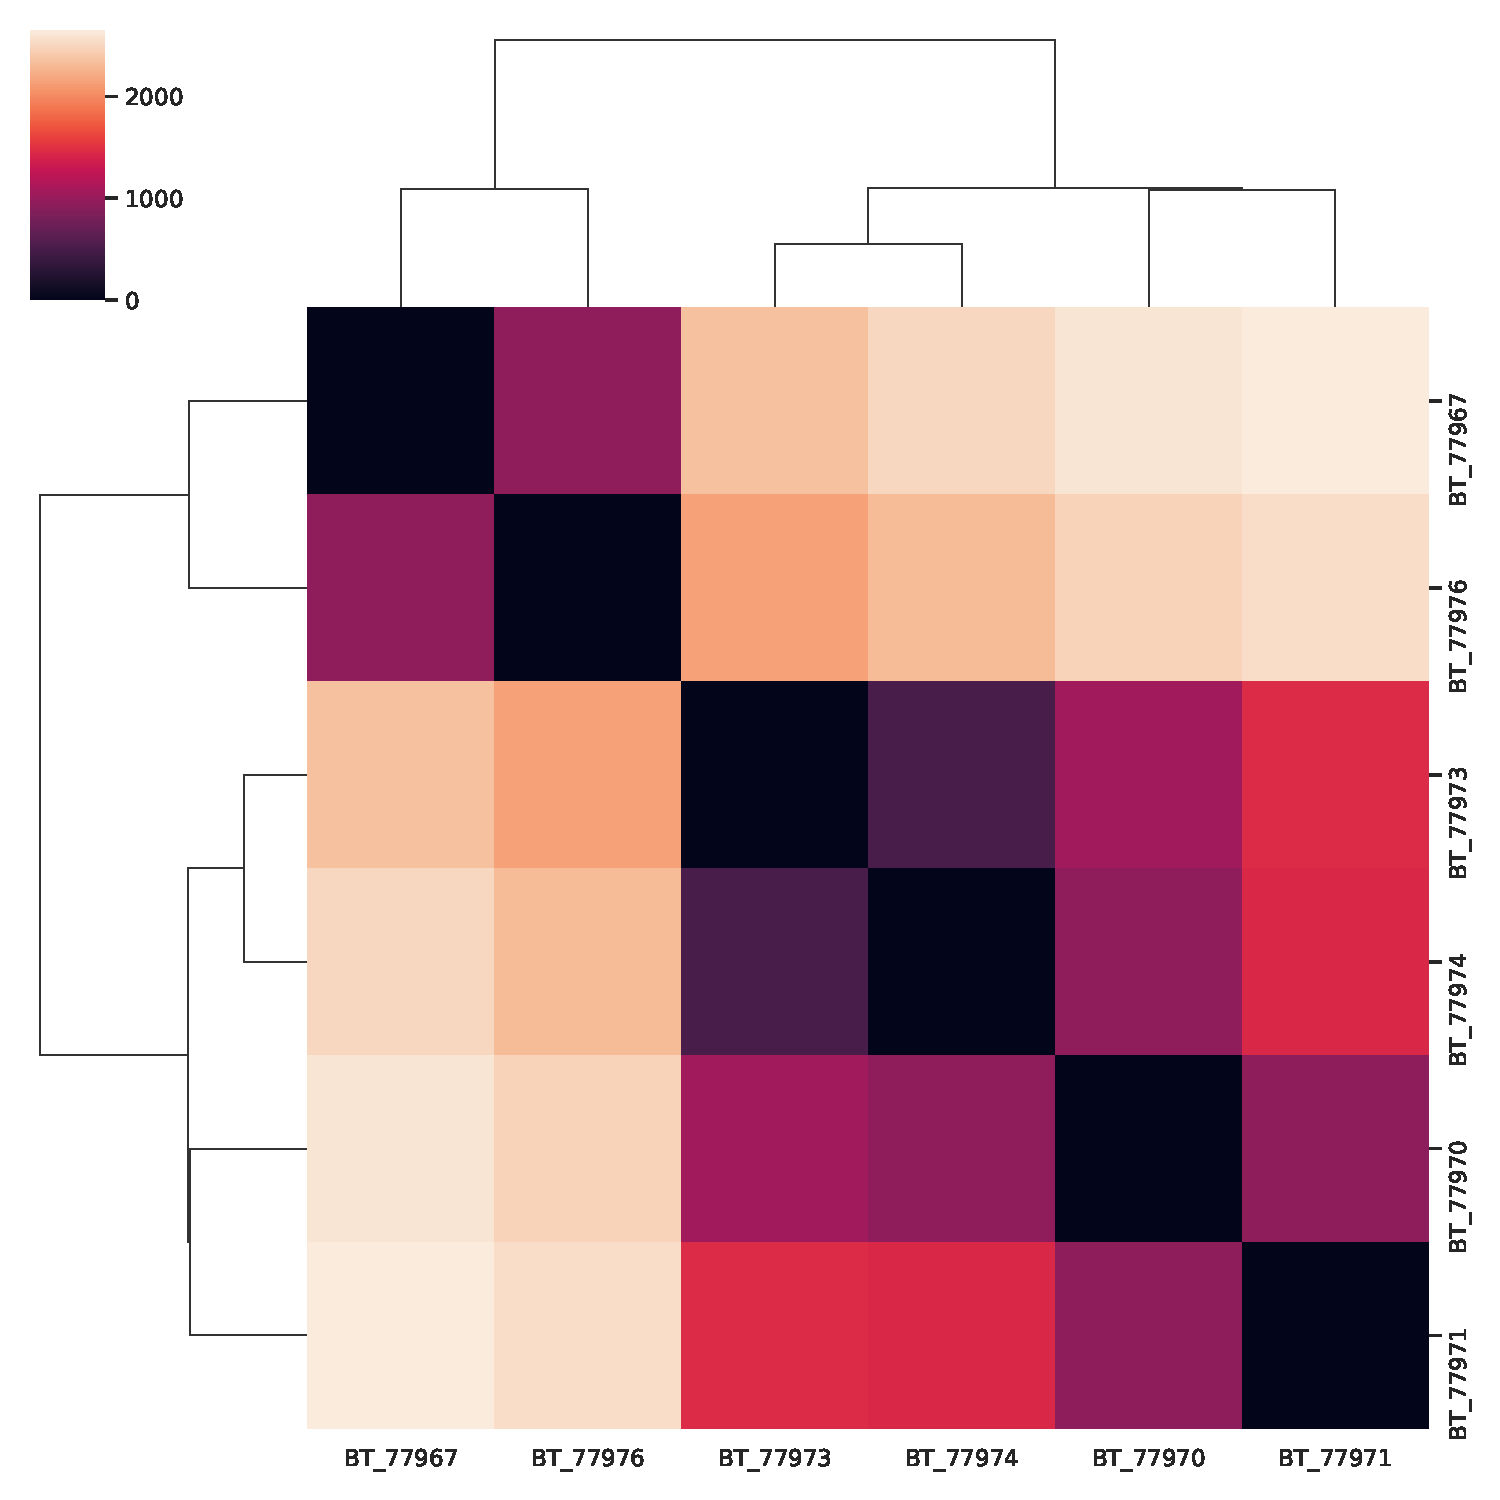
\includegraphics[scale=0.35]{clusters/wasserstein_h2_bt.pdf}
  \caption{\label{fig:label} }
\end{figure}
% The volumes of the eight same we find.

% \begin{figure}[ht]
%   \centering
%   \begin{subfigure}{.249 \linewidth}
%     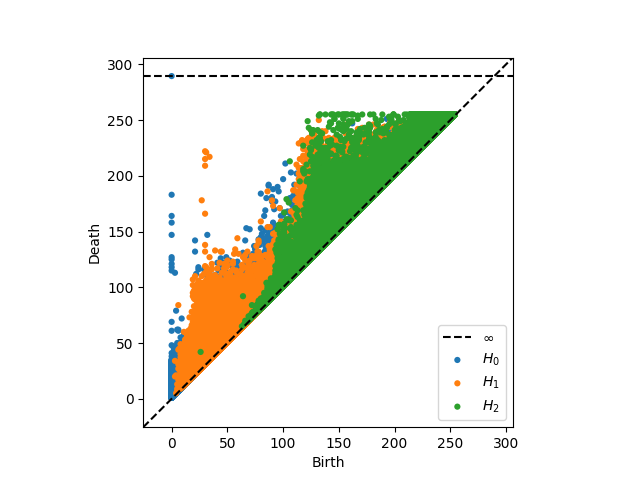
\includegraphics[scale=0.25]{persistence_diagrams/60185_multi_ph.png}
%   \end{subfigure}%
%   \begin{subfigure}{.249 \linewidth}
%     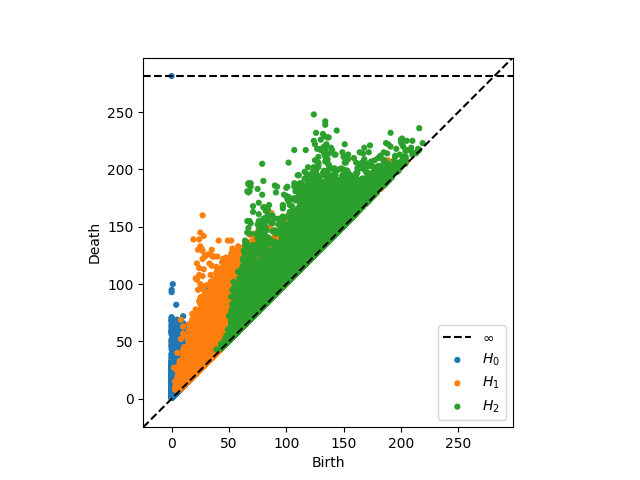
\includegraphics[scale=0.25]{persistence_diagrams/60186_multi_ph.png}
%   \end{subfigure}%
%   \begin{subfigure}{.249 \linewidth}
%     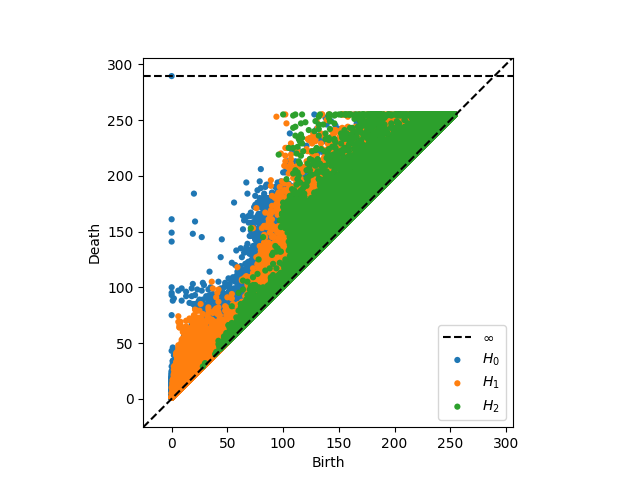
\includegraphics[scale=0.25]{persistence_diagrams/77066_multi_ph.png}
%   \end{subfigure}%
%   \begin{subfigure}{.249 \linewidth}
%     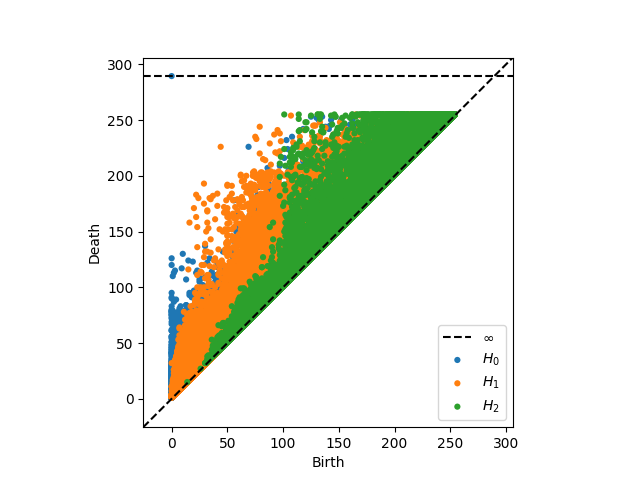
\includegraphics[scale=0.25]{persistence_diagrams/77967_multi_ph.png}
%   \end{subfigure}
%   \begin{subfigure}{.249 \linewidth}
%     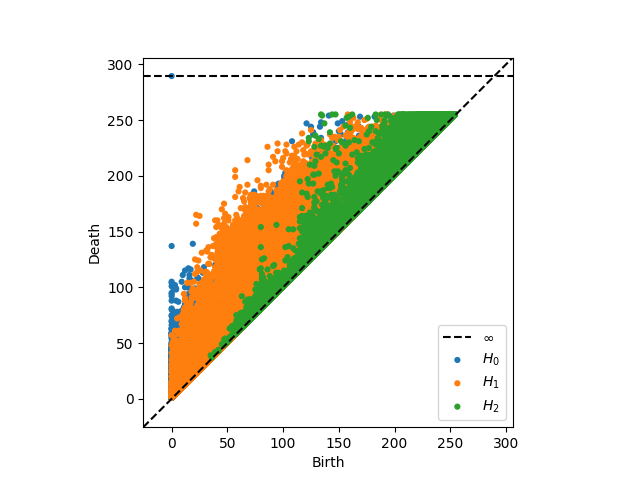
\includegraphics[scale=0.25]{persistence_diagrams/77970_multi_ph.png}
%   \end{subfigure}%
%   \begin{subfigure}{.249 \linewidth}
%     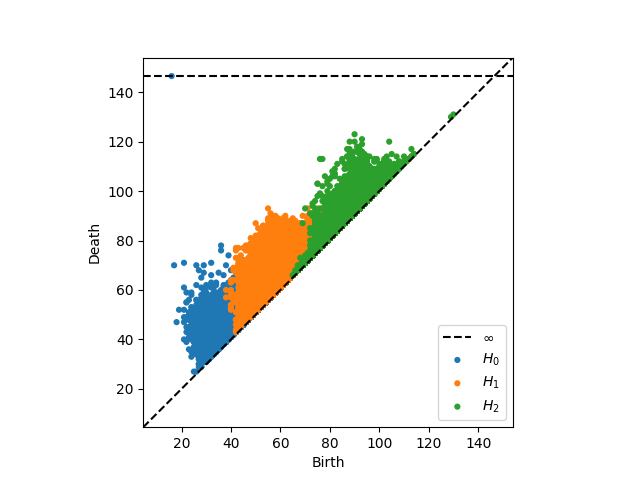
\includegraphics[scale=0.25]{persistence_diagrams/77971_multi_ph.png}
%   \end{subfigure}%
%   \begin{subfigure}{.249 \linewidth}
%     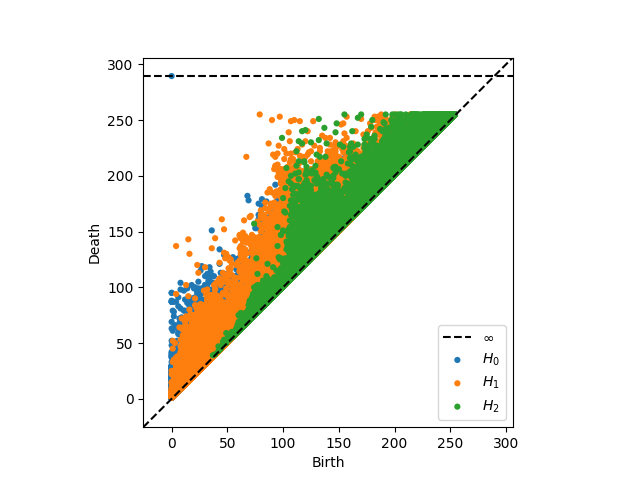
\includegraphics[scale=0.25]{persistence_diagrams/77973_multi_ph.png}
%   \end{subfigure}%
%   \begin{subfigure}{.249 \linewidth}
%     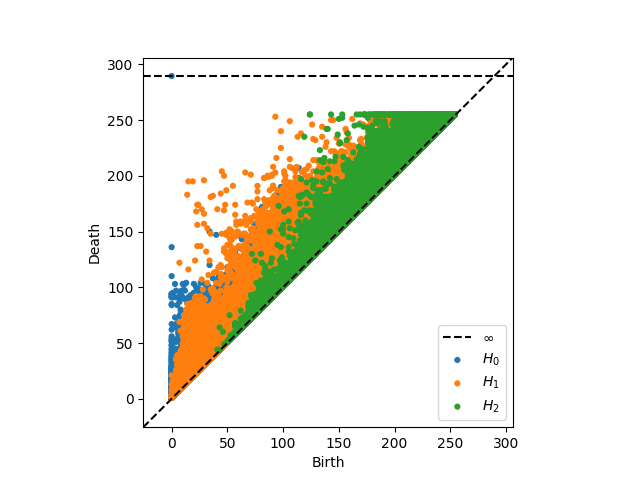
\includegraphics[scale=0.25]{persistence_diagrams/77974_multi_ph.png}
%   \end{subfigure}%
%   \caption{Persistence diagrams of the left eye of the eight bee samples.}
% \end{figure}

% \begin{figure}[ht]
%   \centering
%   \begin{subfigure}{.5 \linewidth}
%     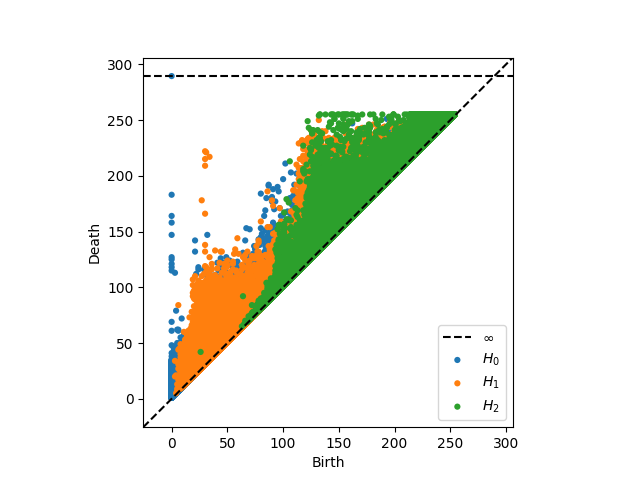
\includegraphics[scale=0.45]{persistence_diagrams/60185_multi_ph.png}
%     \caption{60185}
%   \end{subfigure}%
%   \begin{subfigure}{.5 \linewidth}
%     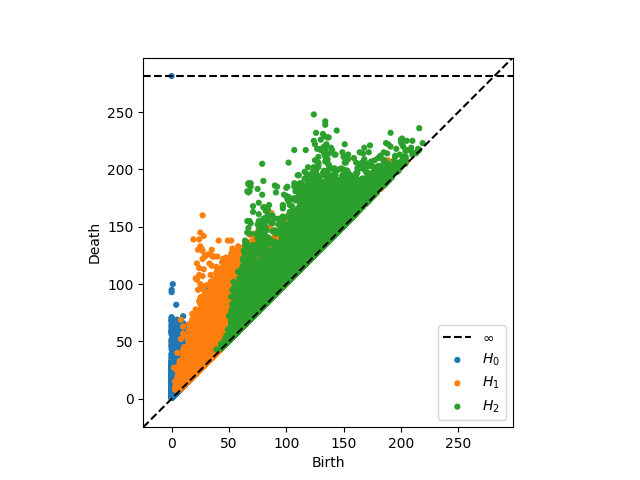
\includegraphics[scale=0.45]{persistence_diagrams/60186_multi_ph.png}
%     \caption{60186}
%   \end{subfigure}
%   \begin{subfigure}{.5 \linewidth}
%     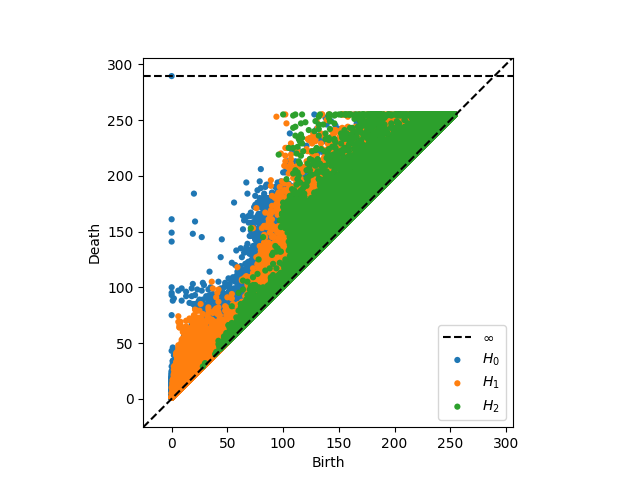
\includegraphics[scale=0.45]{persistence_diagrams/77066_multi_ph.png}
%     \caption{77066}
%   \end{subfigure}%
%   \begin{subfigure}{.5 \linewidth}
%     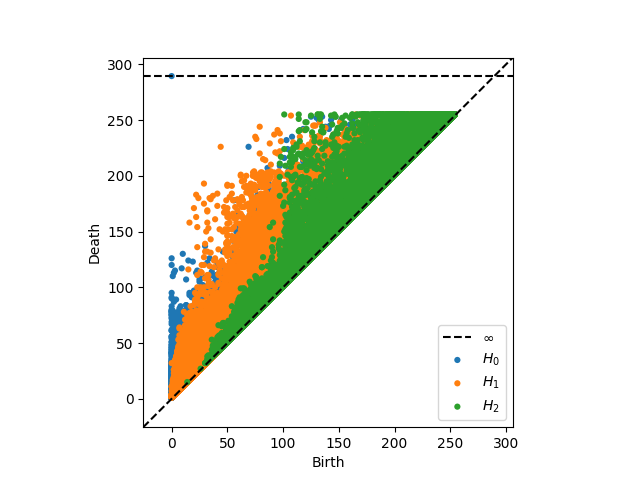
\includegraphics[scale=0.45]{persistence_diagrams/77967_multi_ph.png}
%     \caption{77967}
%   \end{subfigure}
%   \begin{subfigure}{.5 \linewidth}
%     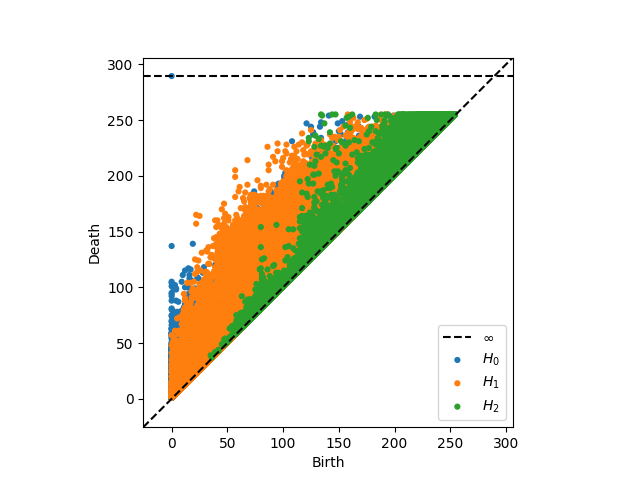
\includegraphics[scale=0.45]{persistence_diagrams/77970_multi_ph.png}
%     \caption{77970}
%   \end{subfigure}%
%   \begin{subfigure}{.5 \linewidth}
%     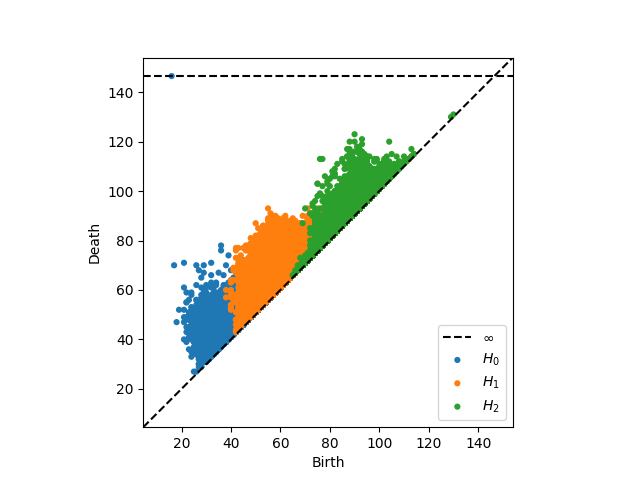
\includegraphics[scale=0.45]{persistence_diagrams/77971_multi_ph.png}
%     \caption{77971}
%   \end{subfigure}
%   \begin{subfigure}{.5 \linewidth}
%     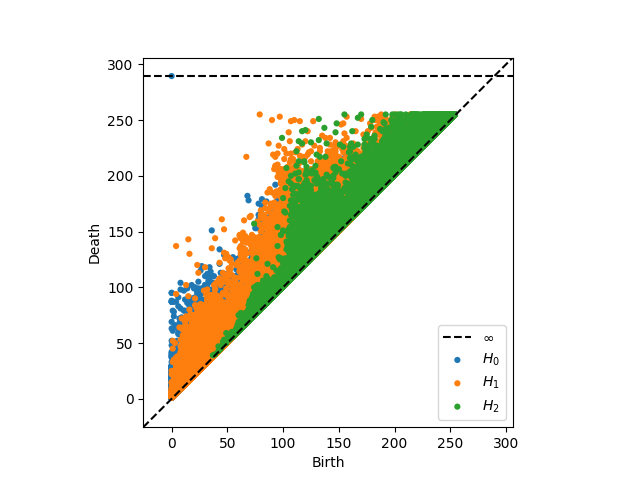
\includegraphics[scale=0.45]{persistence_diagrams/77973_multi_ph.png}
%     \caption{77973}
%   \end{subfigure}%
%   \begin{subfigure}{.5 \linewidth}
%     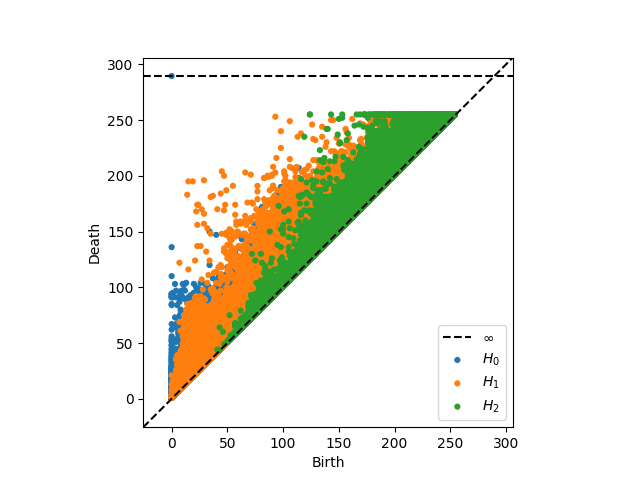
\includegraphics[scale=0.45]{persistence_diagrams/77974_multi_ph.png}
%     \caption{77974}
%   \end{subfigure}
%   \caption{Persistence diagrams of the left eye of the eight bee samples.}
% \end{figure}

% For the graph and heatmaps we have encoded the MorphoSource scan IDs according to the following scheme:
% \begin{center}
% \begin{tabular}{ |c|c| }
%  \hline
%   MorphoSource ID & Encoded ID \\
%   \hline
%  77967 & 0  \\
%  60186 & 1  \\
%  60185 & 2  \\
%  77066 & 3  \\
%  77974 & 4  \\
%  77971 & 5  \\
%  77973 & 6  \\
%  77970 & 7  \\
%  \hline
% \end{tabular}
% \end{center}

% \begin{figure}[ht]
%   \centering
%   \begin{subfigure}{.33 \linewidth}
%     \fbox{
%       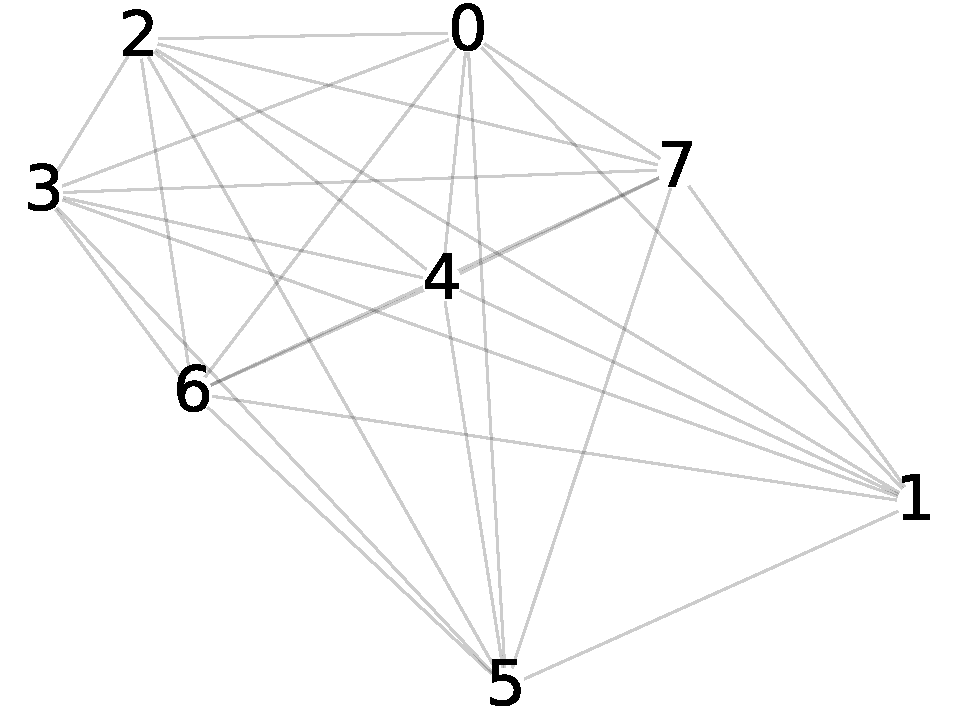
\includegraphics[scale=0.25]{persistence_diagrams/distances/graphs/bottleneck_h0_graph.pdf}
%       }
%   \end{subfigure}%
%   \begin{subfigure}{.33 \linewidth}
%     \fbox{
%       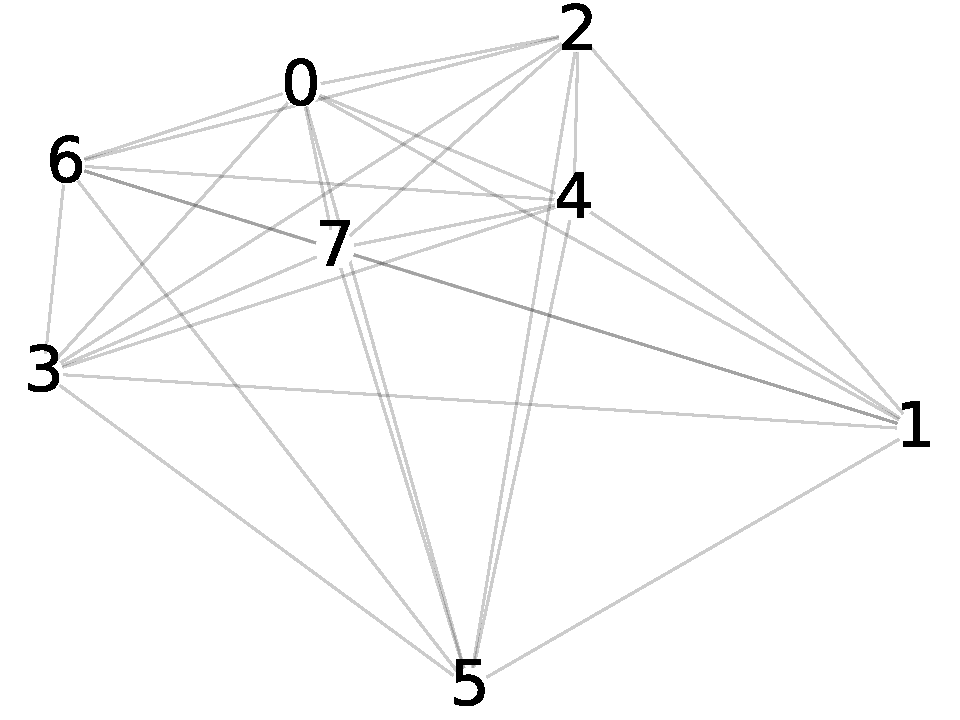
\includegraphics[scale=0.25]{persistence_diagrams/distances/graphs/bottleneck_h1_graph.pdf}
%       }
%   \end{subfigure}%
%   \begin{subfigure}{.33 \linewidth}
%     \fbox{
%     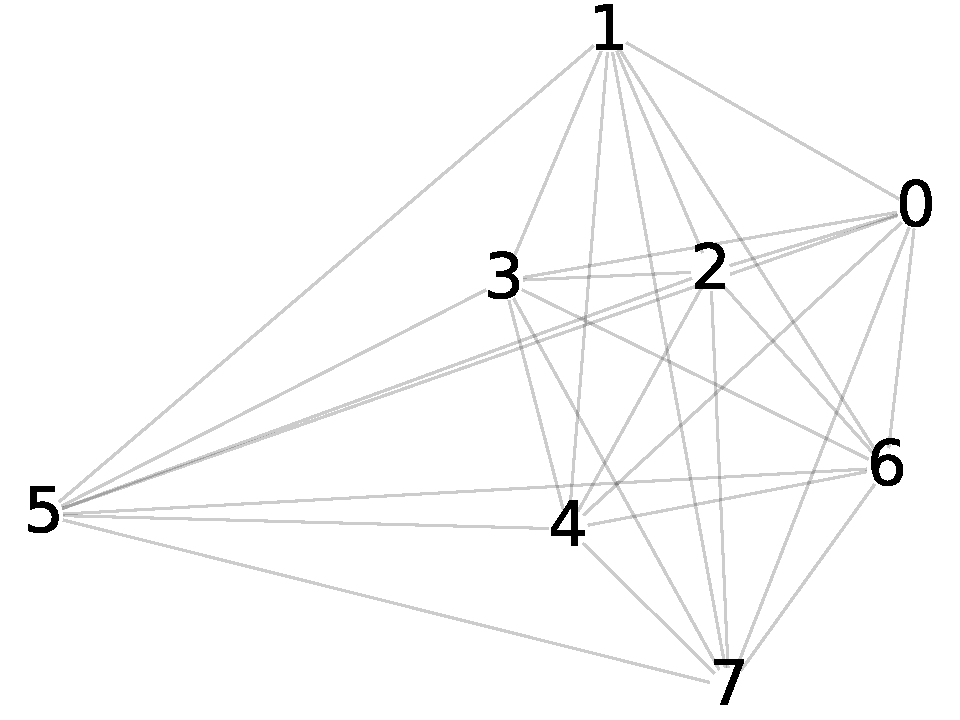
\includegraphics[scale=0.25]{persistence_diagrams/distances/graphs/bottleneck_h2_graph.pdf}
%     }
%   \end{subfigure}

%   \begin{subfigure}{.33 \linewidth}
%     \fbox{
%     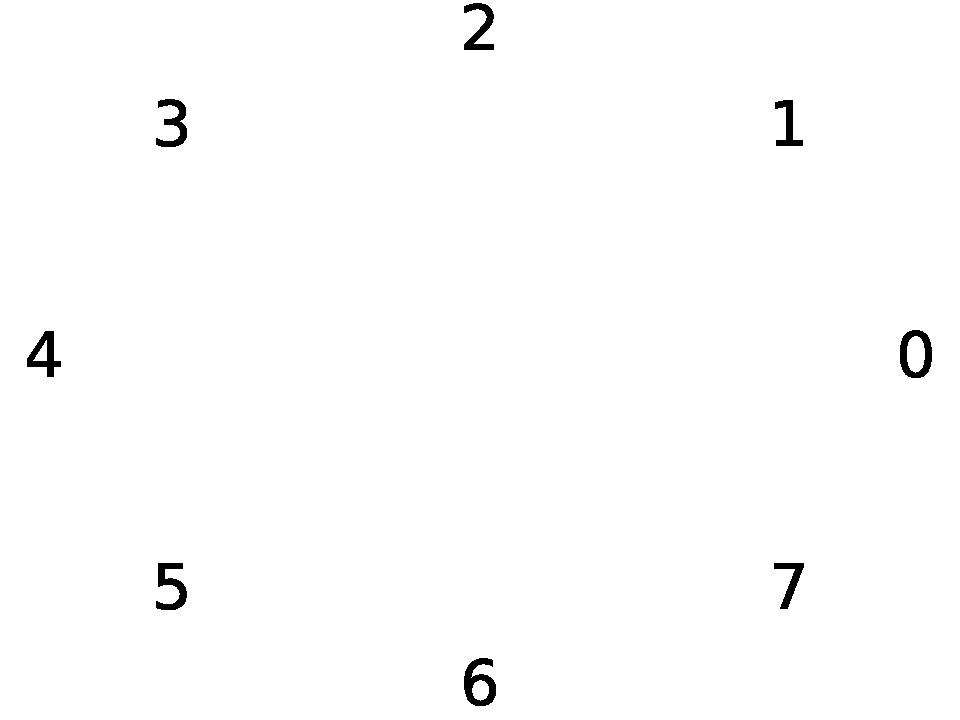
\includegraphics[scale=0.25]{persistence_diagrams/distances/graphs/wasserstein_h0_graph.pdf}
%     }
%   \end{subfigure}%
%   \begin{subfigure}{.33 \linewidth}
%     \fbox{
%     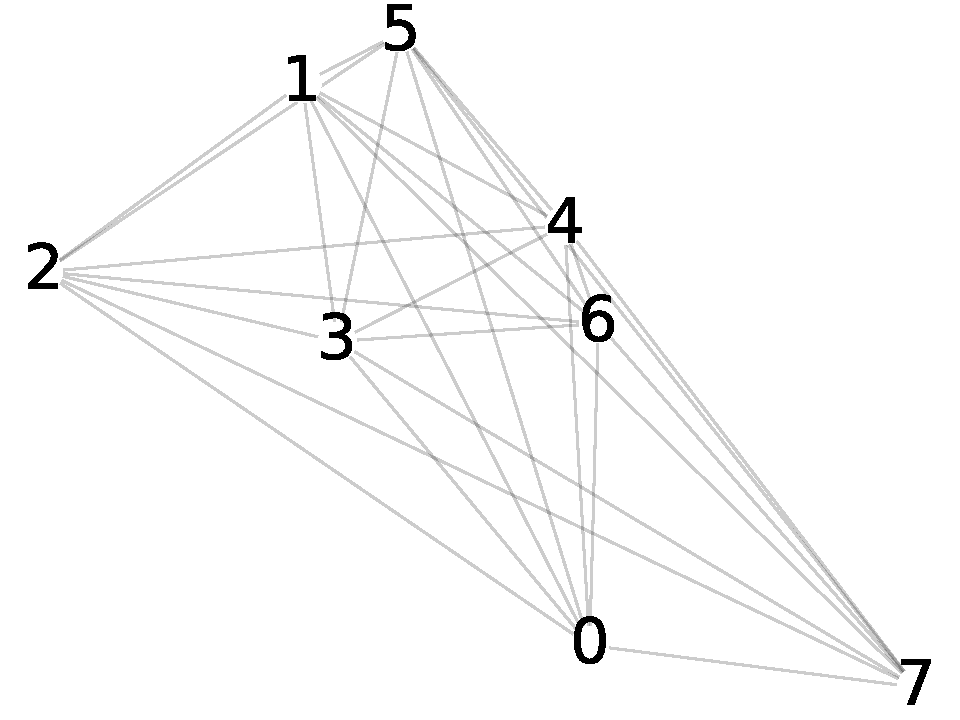
\includegraphics[scale=0.25]{persistence_diagrams/distances/graphs/wasserstein_h1_graph.pdf}
%     }
%   \end{subfigure}%
%   \begin{subfigure}{.33 \linewidth}
%     \fbox{
%     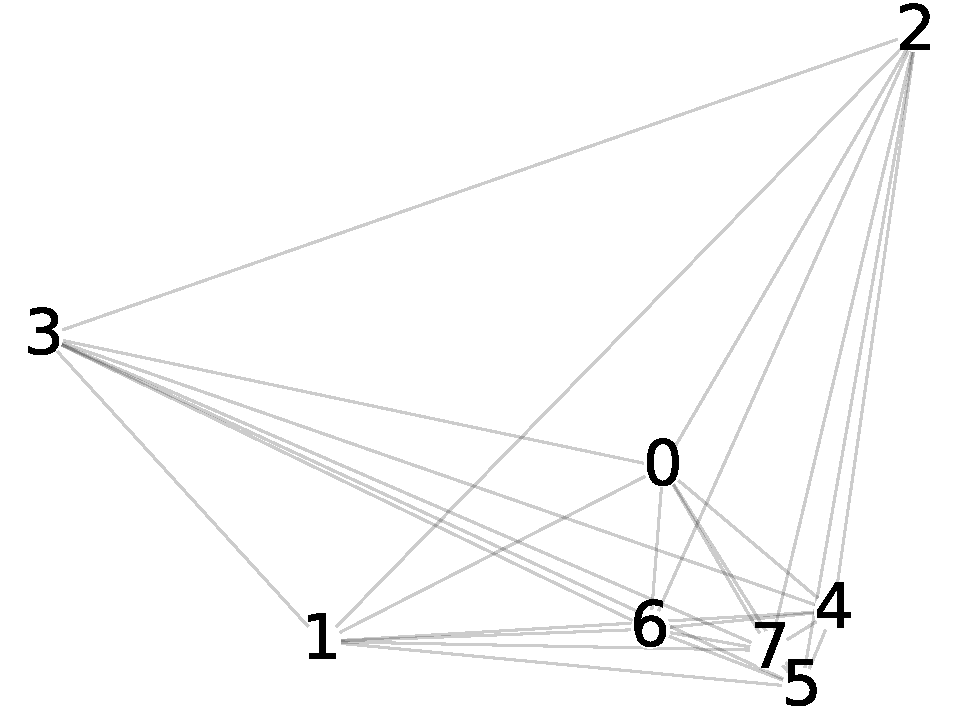
\includegraphics[scale=0.25]{persistence_diagrams/distances/graphs/wasserstein_h2_graph.pdf}
%     }
%   \end{subfigure}%
%   \caption{Graphs that illustrates the pairwise bottleneck distance (top) and pairwise Wasserstein distance (bottom) between the persistence diagrams in $H_{0}, H_{1}, H_{2}$ (left, middle, right) of the bee eyes. Closer nodes indicate more similar persistence diagrams.}
% \end{figure}

% \begin{figure}[ht]
%   \centering
%   \begin{subfigure}{.32 \linewidth}
%     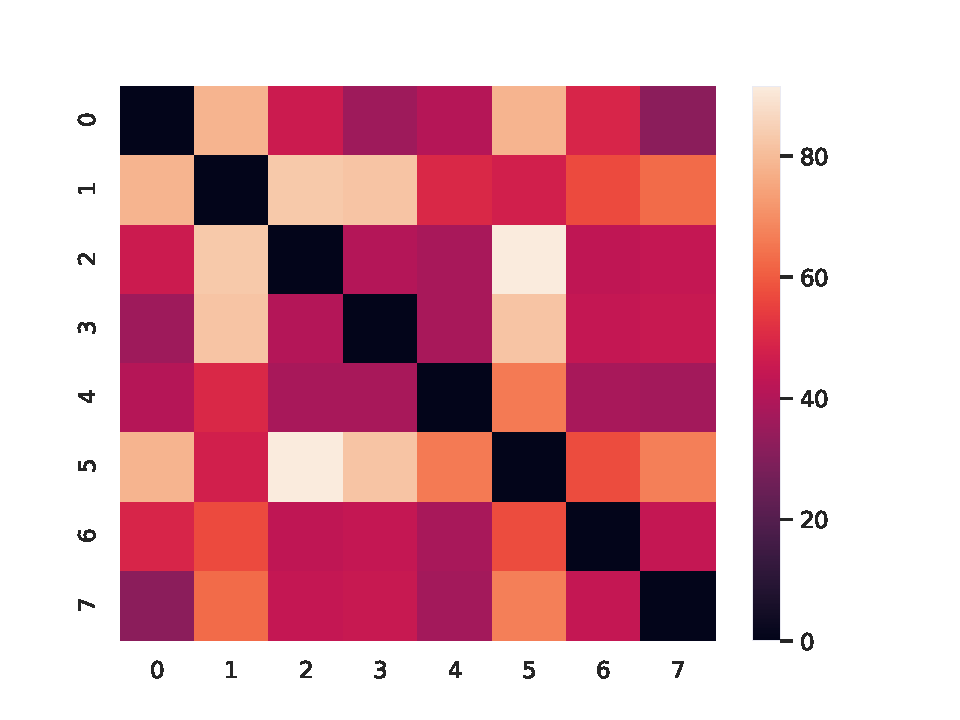
\includegraphics[scale=0.33]{persistence_diagrams/distances/heatmaps/bottleneck_h0.npy.pdf}
%   \end{subfigure}%
%   \begin{subfigure}{.32 \linewidth}
%     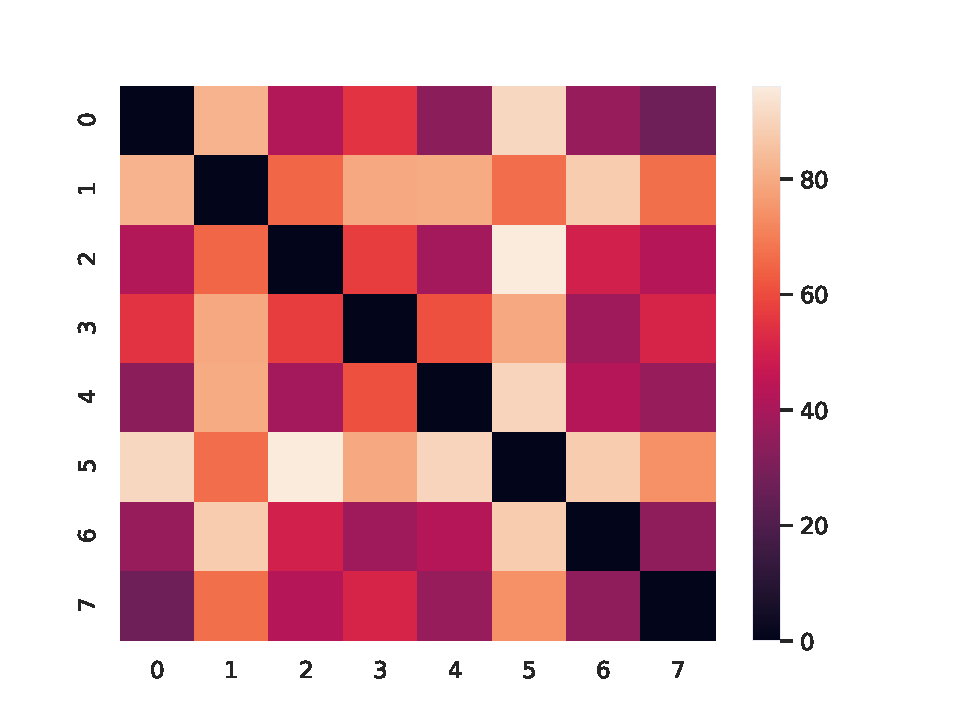
\includegraphics[scale=0.33]{persistence_diagrams/distances/heatmaps/bottleneck_h1.npy.pdf}
%   \end{subfigure}%
%   \begin{subfigure}{.32 \linewidth}
%     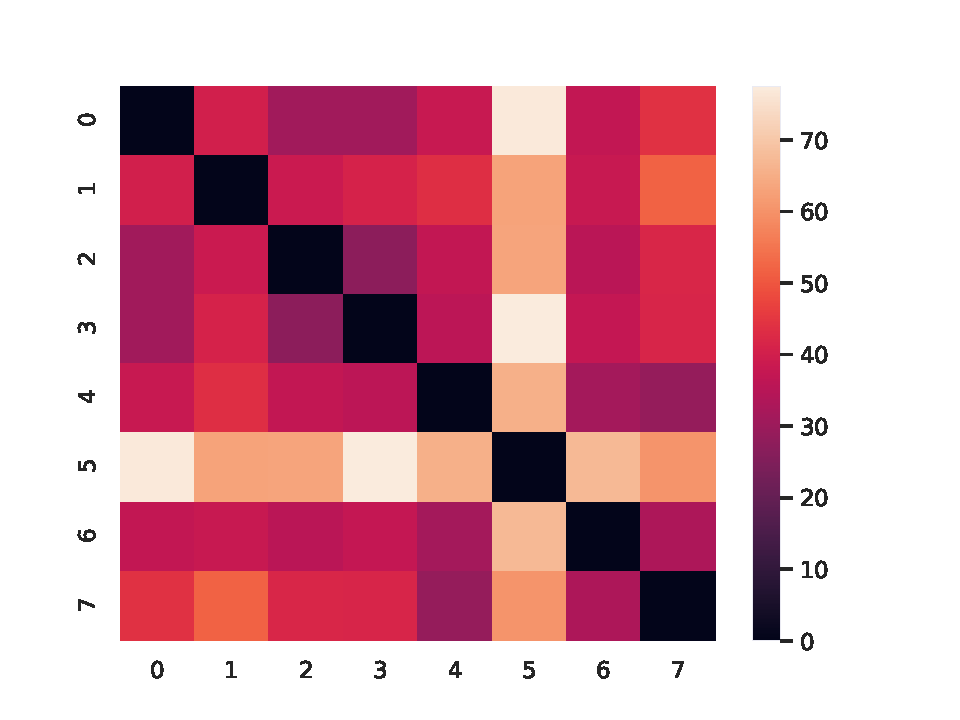
\includegraphics[scale=0.33]{persistence_diagrams/distances/heatmaps/bottleneck_h2.npy.pdf}
%   \end{subfigure}

%   \begin{subfigure}{.32 \linewidth}
%     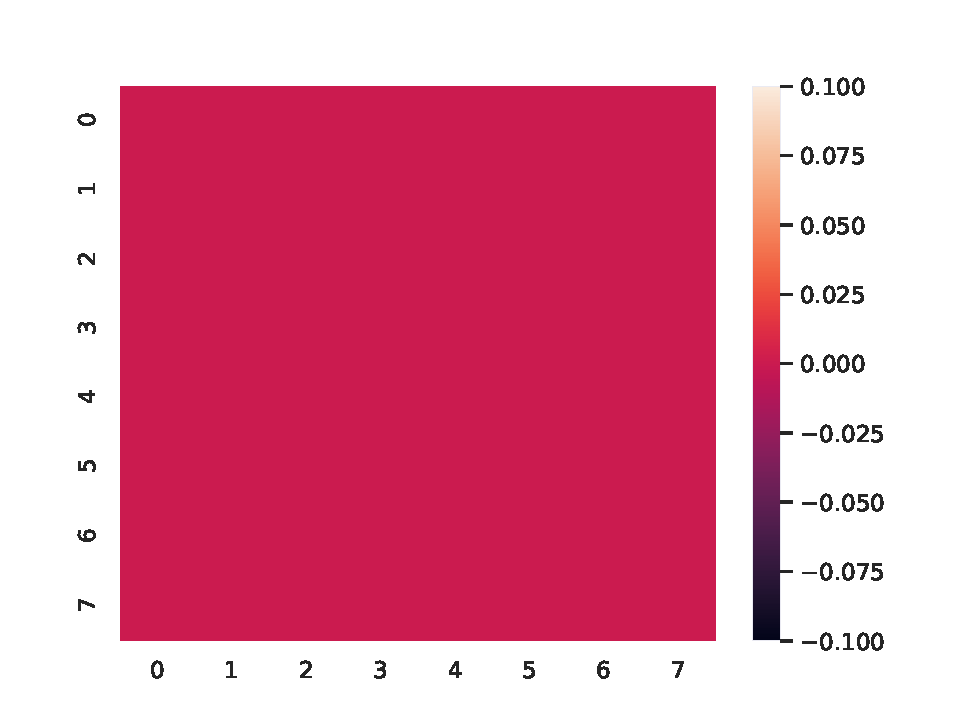
\includegraphics[scale=0.33]{persistence_diagrams/distances/heatmaps/wasserstein_h0.npy.pdf}
%   \end{subfigure}%
%   \begin{subfigure}{.32 \linewidth}
%     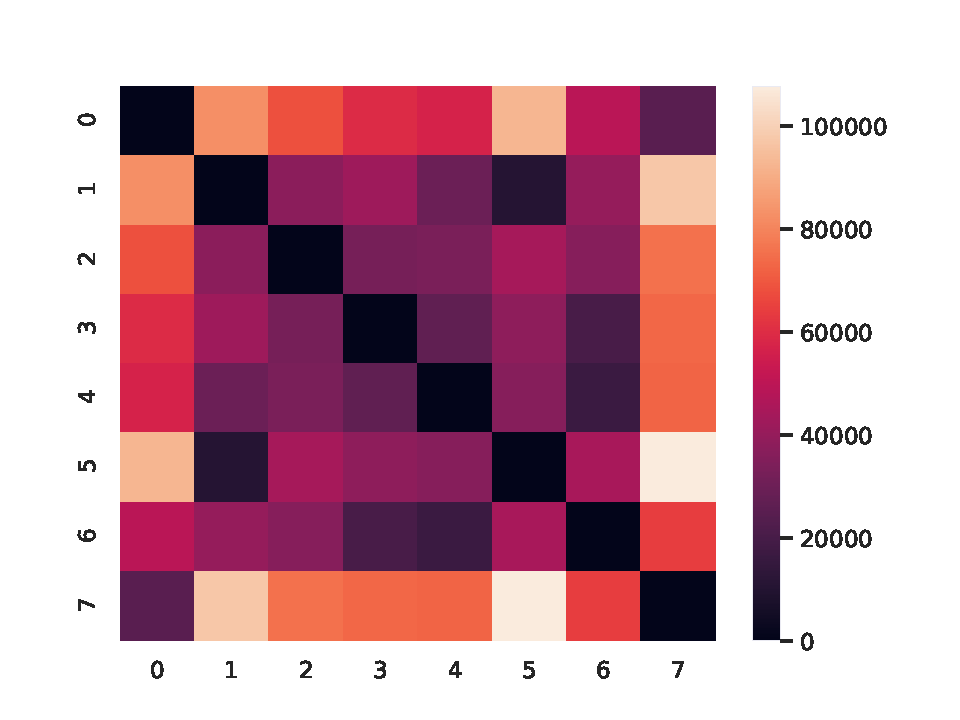
\includegraphics[scale=0.33]{persistence_diagrams/distances/heatmaps/wasserstein_h1.npy.pdf}
%   \end{subfigure}%
%   \begin{subfigure}{.32 \linewidth}
%     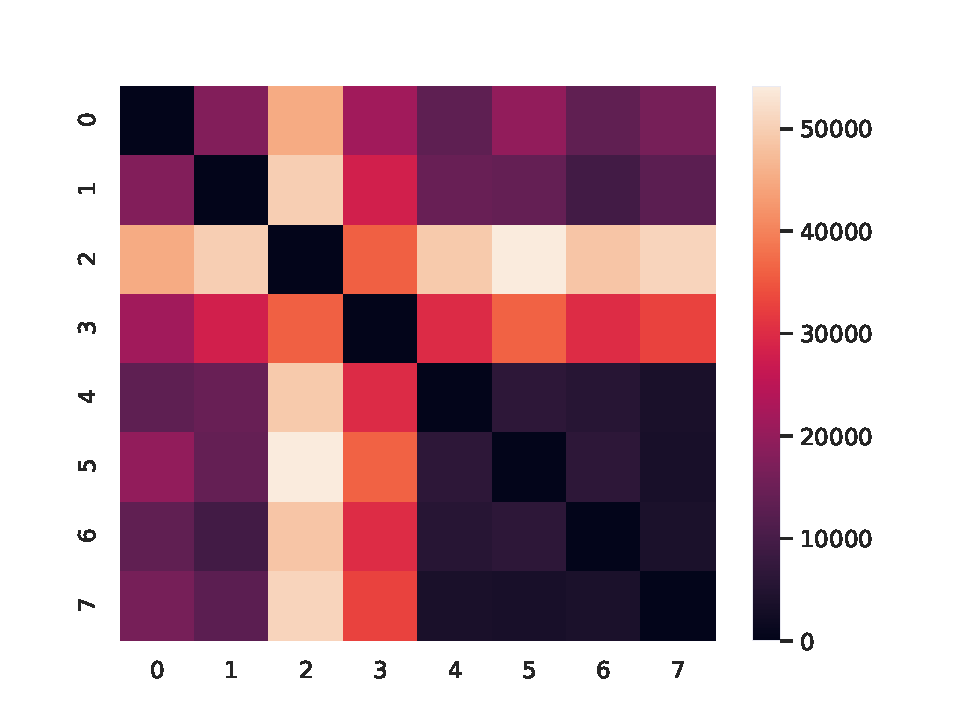
\includegraphics[scale=0.33]{persistence_diagrams/distances/heatmaps/wasserstein_h2.npy.pdf}
%   \end{subfigure}%
%   \caption{Heatmaps that illustrates the pairwise bottleneck distance (top) and pairwise Wasserstein distance (bottom) between the persistence diagrams in $H_{0}, H_{1}, H_{2}$ (left, middle, right) of the bee eyes. Cooler colors indicate closer distance between persistence diagrams.}
% \end{figure}
\clearpage
\section{Brain network (work in progress)}
(WIP)
In this case analysis our main object of study will be two synthetic networks generated based on the striatum.
One network consists of 50 001 vertices and the other network of 999 vertices. It has to be said that the smaller network suffers from being too small to give even the most central neurons all the neighbours it should have.
\begin{definition}
A directed clique is a directed graph $G=(V,E)$ such that every vertex has at least an outgoing or incoming edge to every other vertex in the graph. \end{definition}

\begin{definition}
  Let G=(V,E) be a directed graph. The directed flag complex dFl(G) is defined to be the ordered simplicial complex whose $k$-simplicies are all directed cliques with vertices $v_{0},\dots,v_{k}$ such that $\forall i: v_{i} \in V$
  and $\forall i,j: i < j \implies (v_{i}, v_{j}) \in E$. The vertices $v_{0}, v_{k}$ are called the source and the sink of a $k$-simplex.
\end{definition}

% \begin{tikzpicture}
	\begin{pgfonlayer}{nodelayer}
		\node [style=new style 0] (0) at (-9.5, 0) {$v_0$};
		\node [style=new style 0] (1) at (-1.25, 0) {};
		\node [style=new style 0] (2) at (-1.25, 0) {$v_3$};
		\node [style=new style 0] (3) at (-5.25, 2) {$v_2$};
		\node [style=new style 0] (4) at (-5.25, -1.75) {$v_1$};
		\node [style=none] (5) at (-9.5, 1) {Source};
		\node [style=none] (6) at (-1.25, 1) {Sink};
		\node [style=new style 0] (7) at (1.25, 0) {$v_0$};
		\node [style=new style 0] (8) at (9.5, 0) {};
		\node [style=new style 0] (9) at (9.5, 0) {$v_3$};
		\node [style=new style 0] (10) at (5.5, 2) {$v_2$};
		\node [style=new style 0] (11) at (5.5, -1.75) {$v_1$};
	\end{pgfonlayer}
	\begin{pgfonlayer}{edgelayer}
		\draw [style=new edge style 0] (0) to (3);
		\draw [style=new edge style 0] (0) to (4);
		\draw [style=new edge style 0] (0) to (2);
		\draw [style=new edge style 0] (4) to (2);
		\draw [style=new edge style 0] (4) to (3);
		\draw [style=new edge style 0] (3) to (2);
		\draw [style=new edge style 0] (7) to (11);
		\draw [style=new edge style 0] (7) to (9);
		\draw [style=new edge style 0] (11) to (9);
		\draw [style=new edge style 0] (11) to (10);
		\draw [style=new edge style 0] (10) to (9);
		\draw [style=new edge style 6] (10) to (7);
	\end{pgfonlayer}
\end{tikzpicture}

\begin{figure}[ht]
  \centering
  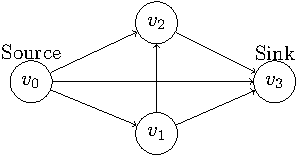
\includegraphics[]{./counts/3simplex.pdf}
  \caption{\label{fig:label} A 3-simplex in a directed flag complex.}
\end{figure}


\begin{figure}[ht]
  \centering
  \begin{subfigure}{.49 \linewidth}
    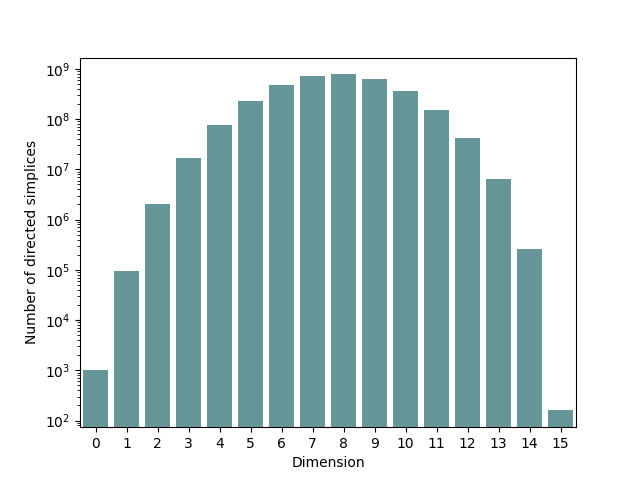
\includegraphics[scale=0.49]{./counts/real1k_count.png}
  \end{subfigure}%
  \begin{subfigure}{.49 \linewidth}
    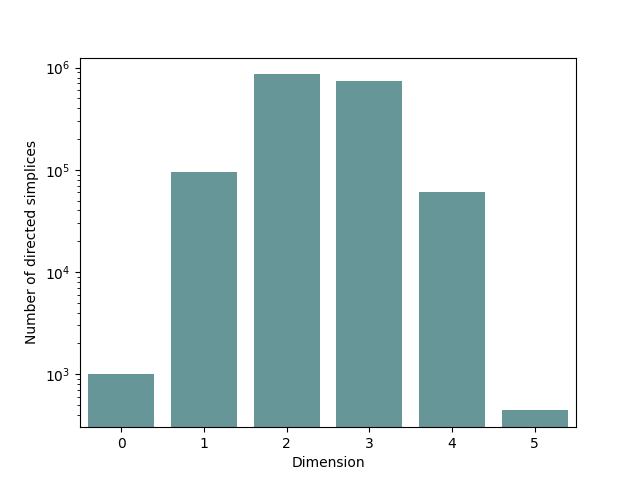
\includegraphics[scale=0.49]{./counts/random1k_count.png}
  \end{subfigure}%
  \caption{\label{count1k}The number of simplices in each dimension for the directed flag complex generated by (a) synthetic network from Snudda, (b) random network generated with the same edge probability creation as the first network, both with 999 vertices.}
\end{figure}

\begin{figure}[ht]
  \centering
  \begin{subfigure}{.49 \linewidth}
    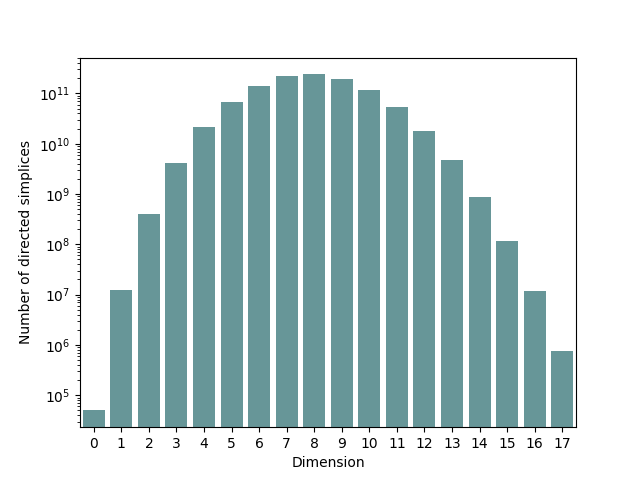
\includegraphics[scale=0.49]{./counts/real50k_count.png}
  \end{subfigure}%
  \begin{subfigure}{.49 \linewidth}
    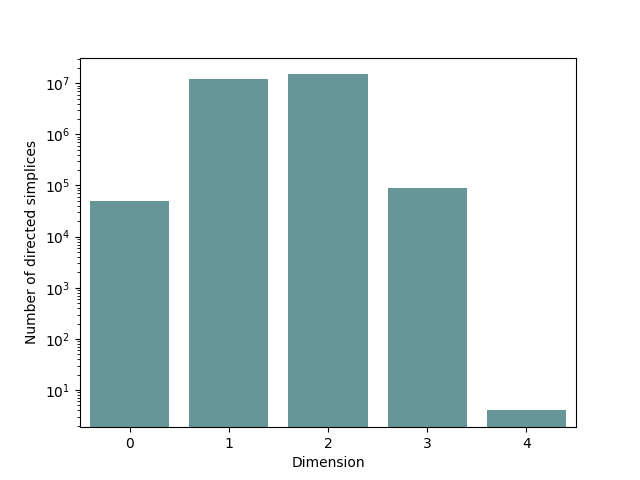
\includegraphics[scale=0.49]{./counts/random50k_count.png}
  \end{subfigure}%
  \caption{\label{count50k}The number of simplices in each dimension for the directed flag complex generated by (a) synthetic network from Snudda, (b) random network generated with the same edge probability creation as the first network, both with 50 001 vertices.}
\end{figure}

In Figures \ref{count1k} and \ref{count50k} we see that the synthetic brain networks have much more higher order structure in terms of high dimensional simplices than a network generated solely based on edge connectivity. For instance, we see in \ref{count50k} the presence of 17-dimensional cells in the synthetic network, which means directed cliques consisting of 18 participating neurons, whereas in the random network we see at most 4-dimensional cell.

In other to further investigate these higher order cells in the synthetic networks we can look at their persistent homology. However, a priori the directed brain network does not have any weights, and so it is not obvious what a filtration $f: V \to \mathbb{R_{+}}$ would look like. So we impose a metric space structure on the directed graph by giving the value of a directed edge between two vertices the Euclidean distance between the two neurons in the simulated model. This means that at low threshold values the filtration will only look at connections made by neurons very close to each other, but as the threshold increases we look at a larger and larger part of the network.

So what is a generator of a homology group in a brain network? It would have to be a $k$-simplex which is not the boundary of a $k+1$-simplex, which translated to the brain network means a clique of neurons that are in themselves an isolated source-sink network and not part of any other network.

Due to computational aspects it is not feasible to compute the persistent homology of the synthetic network with 50 001 vertices, so we restrict ourselves to a subnetwork of the full network consisting only of dSPN neurons as seen in Figure \ref{pers50k}. We also look at a full synthetic network generated with only 999 vertices in Figure \ref{pers1k}.

We see that the formation of higher order $(> 5)$ homology generators mostly happens over small distances, which reaffirms the notion of the brain having a small-world structure.
\begin{figure}[ht]
  \centering
  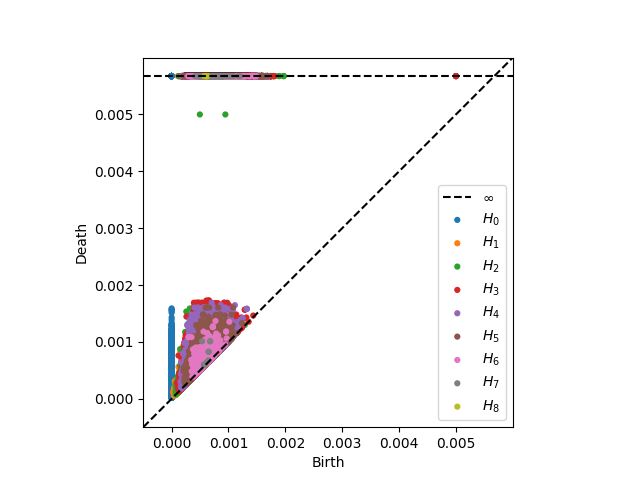
\includegraphics[scale=0.8]{./counts/5kdpsnap10k.png}
  \caption{\label{pers50k} Persistence diagram of the subnetwork of dSPNs extracted from a synthetic network of 50 001 vertices. }
\end{figure}

\begin{figure}[ht]
  \centering
  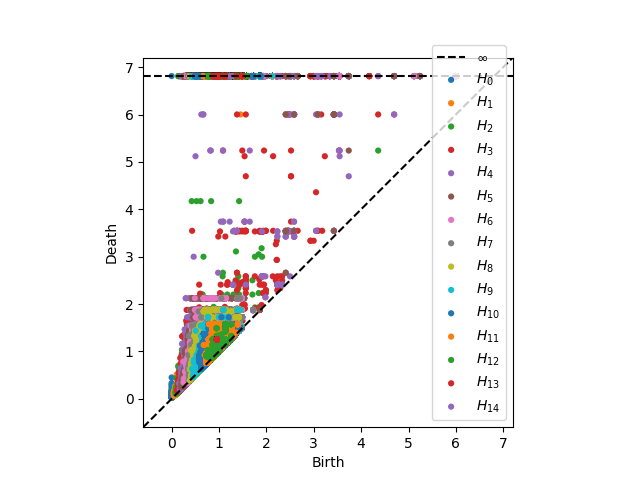
\includegraphics[scale=0.8]{./counts/1kap10000.png}
  \caption{\label{pers1k} Persistence diagram of the entire synthetic network consisting of 999 vertices. (this is scaled 1000 larger than in actual data, generate new diagram)}
\end{figure}
%%% Local Variables:
%%% mode: latex
%%% TeX-master: "thesis.tex"
%%% End:
